\renewcommand{\thefigure}{\textsc{a}\arabic{figure}}
\renewcommand{\theequation}{\textsc{a}\arabic{equation}}
\renewcommand{\thetable}{\textsc{a}\arabic{table}}
\setcounter{figure}{0}
\setcounter{equation}{0}

%\chapter{Appendix to chapter 3}

%\chapter{Appendix to chapter 6}

\chapter{Appendix to chapter 7}

\section{Comment on the simplifications}
\paragraph{Discussion on Simplification (a).}
We ought to remark that, realistically, vaccinations will occur at least eight hours per day. Our assumption, while justified as a computationally convenient approximation of reality, is not a priori worse than assuming that vaccine administration takes place over the whole day. More refined approximations, while in principle possible, pose severe issues because of the nature of the system dynamics. While for most initial values the system dynamics can be easily simulated with time-continuous vaccinations, the system becomes stiff by construction once almost the entire population has been vaccinated. In this case, numerical integration errors can drive the size of some compartments to be negative, which violates the model assumptions and makes the result of the numerical integration meaningless. The main issue in this case is that the optimizer will exploit these inaccuracies in order to reduce the cost. Therefore, this issue is much more evident when solving optimal control problems than when simply simulating the system dynamics. We have investigated some simple approaches to tackle this issue, but no technique yielded satisfactory performances. It is our impression that ad-hoc integration strategies will be required in order to reliably simulate and optimize dynamics with continuous vaccination rates. While this will be the subject of future research, the results obtained with the current approximation have yielded sufficient accuracy.

\paragraph{Discussion on Simplification (b).}
This simplification has been proposed in~\cite{Savorgnan:MultipleShootingDistributed:2011} as an approach to solve distributed optimal control problems by means of multiple shooting. In the original version, the coupling variable $z$ is not necessarily piecewise constant, but rather piecewise polynomial. We have observed in simulations that, for this problem, the piecewise constant parametrization yielded sufficient accuracy.

We discretize the dynamics of each node using an explicit Runge-Kutta integrator of order four, with $50$ integration steps per day. Alternative integrators such as explicit Euler, or implicit Runge-Kutta integrators, yielded similar results. Furthermore, in order to verify the accuracy of the integrator and the impact of the introduced simplifications on the solution accuracy, we simulated the system in open-loop, i.e. we applied the optimal control trajectory to the full model starting from the initial condition provided by the data assimilation scheme.

\paragraph{Discussion on Simplification (c).} We sparsify the mobility matrix by pruning element below a threshold (see Figure \ref{figSI:mobility_simplification}). This operation reduces the number of connection between nodes. Also in this case, we verified through numerical simulations that the introduced simplification had a small impact on the prediction and control accuracy.

\begin{figure*}
\centering
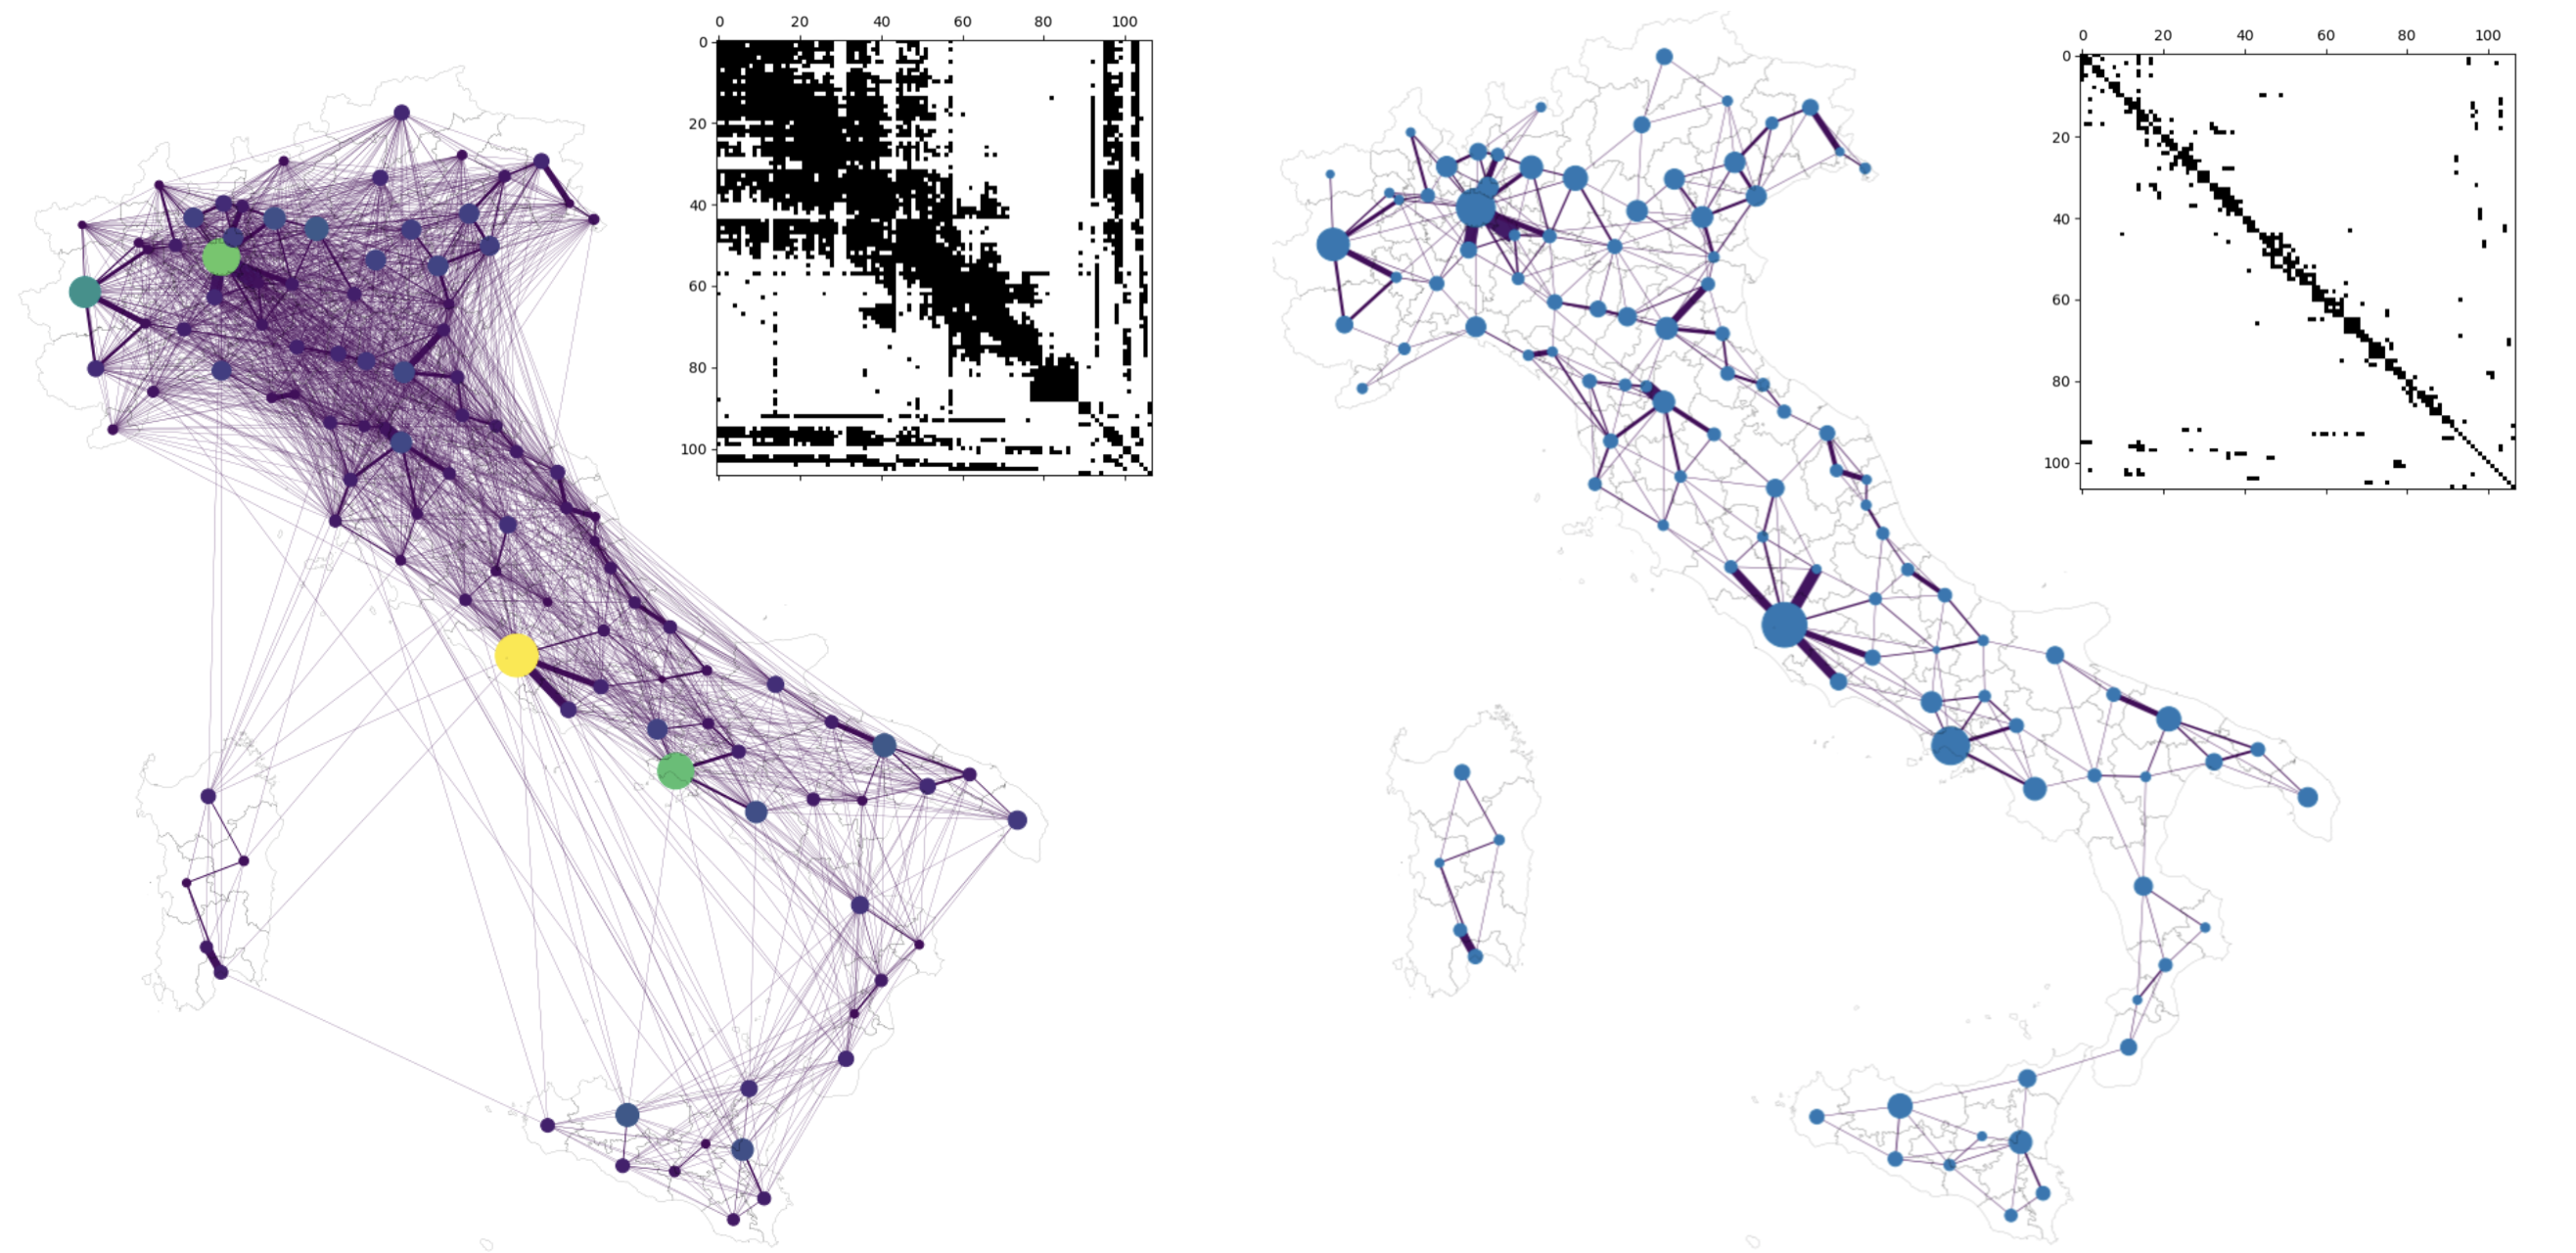
\includegraphics[width=\textwidth]{fig_italy-ocp/figuresSI/mobsimplification.png}
\caption[Simplification of the mobility matrix to obtain a sparse and tractable problem]{Simplification of the mobility matrix to obtain a sparse and tractable problem. After the optimization, we assess the effectiveness of the optimal control strategy on the full model.} \label{figSI:mobility_simplification}
\end{figure*}

\paragraph{Possible further improvements} Applying optimal control in open loop, i.e., solving the optimization problem once and applying the control input over the whole time interval, may lead to poor performance due to model inaccuracy and external perturbations. A common remedy consists in closing the loop by repeatedly solving the OCP by using the most updated information on the initial states. This is the principle behind Model Predictive Control (MPC)~\cite{Rawlings:ModelPredictiveControl:2017}. In this context, the state would be estimated on a daily, weekly, or monthly basis so as to solve again the OCP and correct the optimal strategy.


%% ***********************************************************************************************
%\section{Data assimilation and model parameters}
%% ***********************************************************************************************
%\begin{figure*}
%    \centering
 %   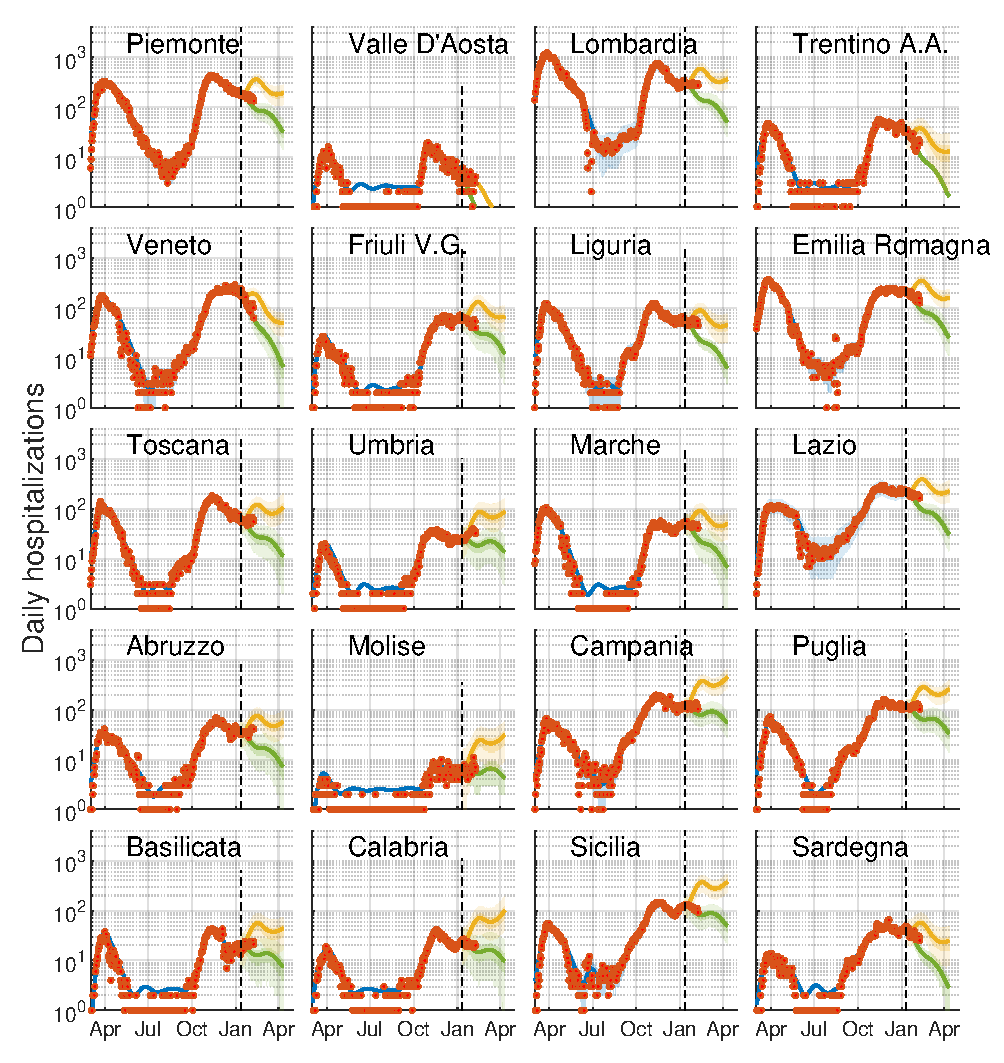
\includegraphics[width=1\textwidth]{fig_italy-ocp/figuresSI/DA_all_sim/hosp.pdf}
  %  \caption[Modeled daily hospitalizations the against hospitalization data]{Modeled daily hospitalizations (blue) versus hospitalization data (red dots), regional detail of Figure 2.A in the main text. The optimistic and pessimistic transmission scenarios are represented in green and yellow, respectively.}
%    \label{fig:SI_DA1}
%\end{figure*}
%\begin{figure*}
%    \centering
%    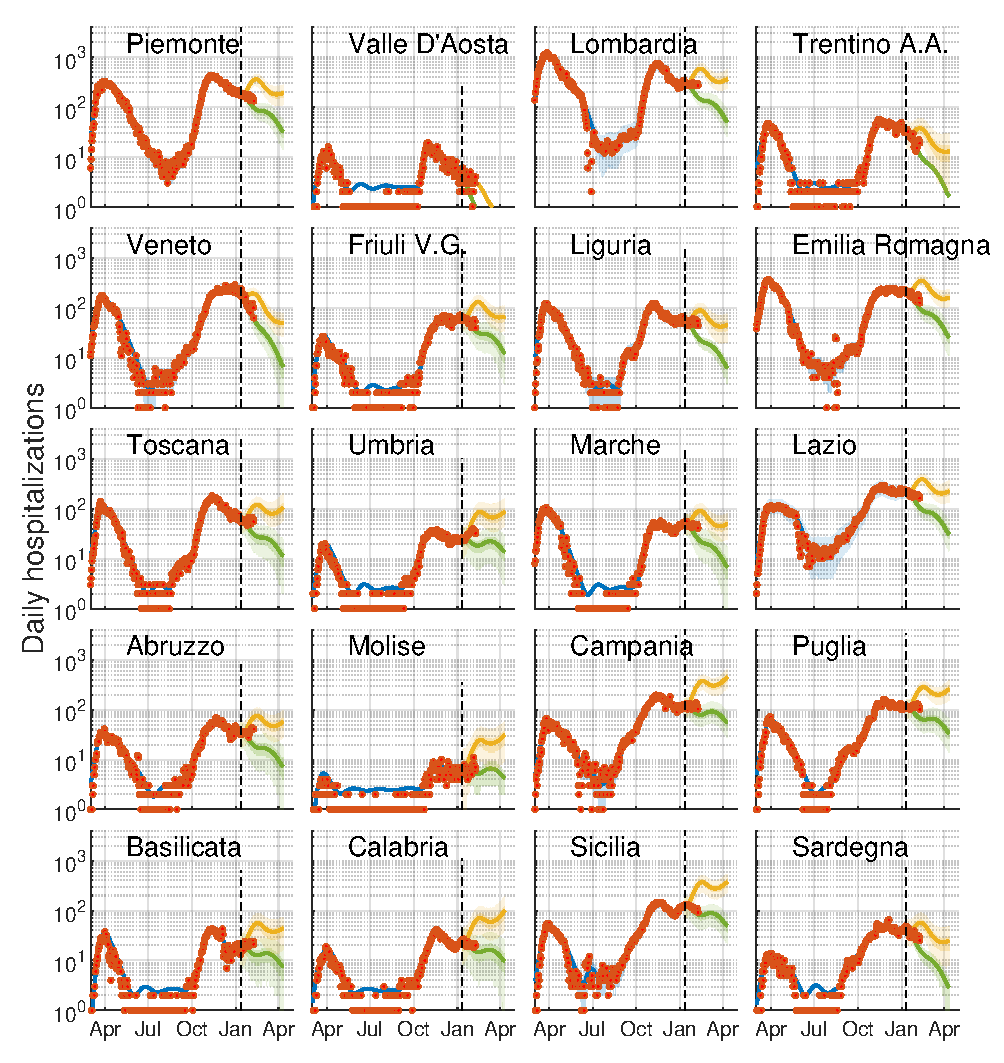
\includegraphics[width=1\textwidth]{fig_italy-ocp/figuresSI/DA_all_sim/incidence.pdf}
%    \caption[Modeled daily incidence against the daily reported cases]{Modeled daily incidence (blue) versus the daily reported cases (red dots), regional detail of Figure 2.B in the main text. The optimistic and pessimistic transmission scenarios are represented in green and yellow, respectively.}
%    \label{fig:SI_DA2}
%\end{figure*}

%The regional transmission rates are the main parameters governing the force of infection of the model and, thus, the daily exposed individuals. To better track possible changes in the transmission rates, we adopt a data assimilation strategy based on an iterative particle filter\cite{Manoli:IterativeParticleFilter:2015} used on a moving window of 14 days. The filter starts considering $N_r=1000$ model realizations at time $t_0$ (February 21st, 2020), whose state variables are $x_0^{(j)}, j=1,\dots, N_r$, where the superscript $(j)$ is the realization index and the subscript is the temporal index. Each realization is associated with a parameter combination that is randomly sampled from the posterior distribution evaluated in\cite{Bertuzzo:GeographyCOVID19Spread:2020}, indicated with $\theta^{(j)}$. Possible spatial heterogeneities in regional transmission on a given day $t_k$ are obtained multiplying the transmission parameter by a coefficient $\phi_{k,i}^{(j)}$, where $i$ is the region's index. At time $t_0$, the coefficients $\phi_{0,i}^{(j)}$ are sampled from a truncated normal distribution (mean $\mu_0=1$, standard deviation 0.4, bounds $0.8\mu$-$1.2\mu_0$).
%At time $t_k$, we assume to know the state variables $x_k^{(j)}$ and coefficients $\phi_{k,i}^{(j)}$, the latter having ensemble mean $\mu_{k,i}$. To update state variables and coefficients at time $t_{k+1}$, we consider the observations (daily hospitalizations) collected in a temporal window of $\tau=14$ days, $(t_k,t_{k}+\tau$. New coefficients from the truncated normal distribution (mean $\mu_k=1$, standard deviation 0.4, bounds $0.8\mu_k$-$1.2\mu_k$) are sampled at time $\tau=t_0+14$ days.  For each realization, we run the model during the window of 14 days, assuming that the coefficients change linearly for a week, from  $\phi_{0,i}^{(j)}$ to $\tilde{\phi}_{0,i}^{(j)}$, and remain constant afterwards.
%The regional likelihood of each realization is then evaluated during these two weeks considering that the daily hospitalizations follow a gamma distribution (as in\cite{Bertuzzo:GeographyCOVID19Spread:2020}). 
%A resampling step (systematic resampling , see, e.g.\cite{Douc:ComparisonResamplingSchemes:2005}) selects and duplicates the coefficients $\tilde{\phi}_{0,i}^{(j)}$ associated with the largest likelihood values. These coefficients are then used to update the mean value $\mu_k$. Finally, the simulation is repeated on the same temporal window by sampling new coefficients $\tilde{\phi}_{0,i}^{(j)}$ from the truncated normal distribution with the updated mean $\mu_k$. This set of coefficients is used to compute state variables and parameters at time $t_k$, and then as starting condition to produce the projections used in the main text.

%Model parameters (in the absence of vaccination) are taken from a paper\cite{Bertuzzo:GeographyCOVID19Spread:2020} where they were inferred in a Bayesian framework for the period February~24th -- May~1st, 2020, on the basis of the official epidemiological bulletins released daily by Dipartimento della Protezione Civile\cite{DipartimentodellaProtezioneCivile:EmergenzaCoronavirusRisposta} (data available online at {\url{https://github.com/pcm-dpc/COVID-19}}) and the bulletins of Epicentro, at Istituto Superiore di Sanit{à}\cite{IstitutoSuperiorediSanita:CoronavirusUltimiAggiornamenti:2020,Palmieri:CharacteristicsCOVID19Patients:2020}. All the parameters estimated for the initial phase of the Italian COVID-19 epidemic, including the transmission rates, are spatially homogeneous\cite{Bertuzzo:GeographyCOVID19Spread:2020}. This parameterization has been used to produce all the results presented in the main text.


%% ***********************************************************************************************
\paragraph{Spatial set-up} 
%% ***********************************************************************************************
The modeling tools described in the following sections are applied to the Italian COVID-19 epidemic at the scale of second-level administrative divisions, i.e. provinces and metropolitan cities (currently, as of 2021, $107$ spatial units). Official data about resident population at the provincial level is produced yearly by the Italian National Institute of Statistics (Istituto Nazionale di Statistica, ISTAT; data available at\\ \url{http://dati.istat.it/Index.aspx?QueryId=18460}). The latest update (January 1, 2019) has been used to inform the spatial distribution of the population. %For the age-stratified model the data also comes from ISTAT, in the 2018 census: \url{http://demo.istat.it/popres/index.php?anno=2018&lingua=eng}.
The data to quantify nation-wide human mobility come from ISTAT (specifically, from the 2011 national census; data available online at \url{https://www.istat.it/it/archivio/139381}). Mobility fluxes, mostly reflecting commuting patterns related to work and study purposes, are provided at the scale of third-level administrative units (municipalities)\cite{Pepe:COVID19OutbreakResponse:2020,Vollmer:Report20Using:2020}. These fluxes were upscaled to the provincial level following the administrative divisions of 2019, and used to evaluate the fraction $p_i$ of mobile people in each node~$i$, as well as the fraction $q_{ij}$ of mobile people who move between~$i$ and all other administrative units~$j$ (see Supplementary Material in\cite{Gatto:SpreadDynamicsCOVID19:2020}).
The epidemiological data is obtained from the bulletins of the Dipartimento della Protezione Civile, \url{https://github.com/pcm-dpc/COVID-19}).

%% ***********************************************************************************************
\section{Details of the alternative strategies}
%% ***********************************************************************************************
We designed alternative strategies to compare the optimal solutions. Each strategy uses a decision variable, $\mathcal{V}_i$, as a basis for the allocation of vaccines among provinces. The decision variable is one of:
\begin{itemize}
    \item \textsc{modelled future incidence, absolute}: the modelled total future incidence in a no-vaccination scenario. This is equivalent to the objective of the optimal control problem with no control;
    \item \textsc{modelled future incidence, per population}: as above, but normalized by the resident population in each node;
    \item \textsc{modelled initial susceptibility, absolute}: the modelled number of susceptibles in each province at the start of the vaccination campaign;
    \item \textsc{modelled initial susceptibility, per population}: as above, but normalized by the resident population in each node;
    \item \textsc{province's population}.
\end{itemize}

We define two strategies to distribute the doses:
\begin{itemize}
\item \textsc{Focused} Where every province is sorted (higher on top) according to its decision variable $\mathcal{V}_i$. We then allocate the maximum local rate $v_i^{max}$ to every province going down through the list, until the stockpile is empty. In other words, assuming we have an amount $K$ of vaccines in the stockpile, we find the province index $i$ that satisfy $\max_i \mathcal{V}_i$, and we assign to province $i$ $M_i = \min(v_i^{max}, K)$ vaccines. Then, we find the province $j$ that satisfy $\max_{j,j\neq i} \mathcal{V}_j$ and we assign it $M_j = \min(v_j^{max}, K-M_i)$. And so on, until no vaccine remains in the stockpile. This strategy will concentrate the allocation on nodes with the highest values of the considered decision variable.
\item \textsc{Proportional} In this case, assuming that on a given day there is a quantity of vaccine $K$ in the stockpile, we assign to each province $i$ an amount $M_i = \min(v_i^{max}, K \cdot \frac{\mathcal{V}_i}{\sum_j \mathcal{V}_j})$. This approach vaccinate each node proportionally to the value of its decision variable $\mathcal{V}_i$.
\end{itemize}
In the main text, we show the results for three alternative strategies, namely \textit{proportional absolute incidence}, \textit{proportional population}, and \textit{proportional susceptibility}---named respectively Incidence, Population, and Susceptibility. These strategy are good performers across scenarios, and show how different choices for the decision variables may affect the outcomes of the OCP. In the next sections, we will show the results for all these alternative strategies.

%% ***********************************************************************************************
\section{Additional results}
%% ***********************************************************************************************
We present the results for all these strategies in Table \ref{table:all_strat}, and we show them side-by-side in Figure \ref{fig:OC_comparison_all}. The optimal solutions outperforms all the others solution. In fact, for every given posterior realisation, the optimal control solution always outperforms all other allocation strategies. Even if we observe some scatter when sampling the posterior, the performances of optimal strategies are clearly separated from the rest of the alternatives.

To further investigate the features of the optimal solution, we present a linear scatter plot of the optimal proportion of vaccinated individuals per province (sorting variable) side by side with the province population, the projected incidence without vaccination, and the proportion of susceptible individuals at the start of the simulation. We present these results for the optimistic scenario in Figure \ref{fig:OC_scatter_optimistic} and for the pessimistic scenario in Figure \ref{fig:OC_scatter_pessimistic}. We find no clear visual pattern associating these covariates to the optimal proportion vaccinated, highlighting again that the optimal allocation uses the epidemiological variable in a non-straightforward way, different from every simple strategy we could come up with.

\begin{fwtable}
\centering
\small
\begin{tabular}{llrrrr}
\toprule
& {} & \multicolumn{2}{c}{Averted Infections} & \multicolumn{2}{c}{Averted Infections} \\
&    &  & & \multicolumn{2}{c}{per dose} \\
Scenario & Method &  Optimistic & Pessimistic &     Optimistic & Pessimistic          \\
\midrule
2M & Optimal &   6.98M &    30.6M &          0.268 &        1.18 \\
        & Incidence &   6.32M &    28.1M &          0.243 &        1.08 \\
        & Proportional Incidence &   6.23M &    27.5M &          0.239 &        1.06 \\
        & Focused Susceptibility &   6.03M &    26.9M &          0.232 &        1.03 \\
        & Focused Proportional Susceptibility &   6.03M &    26.9M &          0.232 &        1.03 \\
        & Focused Proportional Incidence &   6.03M &    26.9M &          0.232 &        1.03 \\
        & Focused Population &   6.03M &    26.9M &          0.232 &        1.03 \\
        & Focused Incidence &   6.03M &    26.9M &          0.232 &        1.03 \\
        & Population &   6.02M &    26.8M &          0.231 &        1.03 \\
        & Susceptibility &   5.97M &    26.7M &          0.229 &        1.02 \\
        & Proportional Susceptibility &    5.6M &    25.3M &          0.215 &       0.971 \\
1.5M & Optimal &   5.52M &    24.1M &          0.283 &        1.24 \\
        & Incidence &   4.89M &    21.7M &           0.25 &        1.11 \\
        & Proportional Incidence &   4.82M &    21.3M &          0.246 &        1.09 \\
        & Focused Population &   4.58M &    20.5M &          0.235 &        1.05 \\
        & Focused Incidence &   4.58M &    20.5M &          0.235 &        1.05 \\
        & Focused Proportional Incidence &   4.58M &    20.5M &          0.235 &        1.05 \\
        & Focused Proportional Susceptibility &   4.58M &    20.5M &          0.235 &        1.05 \\
        & Focused Susceptibility &   4.58M &    20.5M &          0.235 &        1.05 \\
        & Population &   4.57M &    20.4M &          0.234 &        1.05 \\
        & Susceptibility &   4.51M &    20.3M &          0.231 &        1.04 \\
        & Proportional Susceptibility &   4.18M &     19.0M &          0.214 &       0.975 \\
1M & Optimal &    3.9M &    16.9M &            0.3 &         1.3 \\
        & Incidence &   3.41M &    15.1M &          0.262 &        1.16 \\
        & Proportional Incidence &   3.34M &    14.7M &          0.257 &        1.13 \\
        & Focused Population &   3.09M &    13.9M &          0.238 &        1.07 \\
        & Focused Susceptibility &   3.09M &    13.9M &          0.238 &        1.07 \\
        & Focused Proportional Susceptibility &   3.09M &    13.9M &          0.238 &        1.07 \\
        & Focused Incidence &   3.09M &    13.9M &          0.238 &        1.07 \\
        & Focused Proportional Incidence &   3.09M &    13.9M &          0.238 &        1.07 \\
        & Population &   3.08M &    13.8M &          0.237 &        1.06 \\
        & Susceptibility &   3.02M &    13.7M &          0.232 &        1.05 \\
        & Proportional Susceptibility &   2.75M &    12.6M &          0.211 &       0.972 \\
479'700 & Optimal &   1.96M &    8.39M &          0.314 &        1.34 \\
        & Focused Proportional Incidence &   1.95M &    7.74M &          0.312 &        1.24 \\
        & Proportional Incidence &   1.69M &    7.32M &          0.271 &        1.17 \\
        & Incidence &   1.63M &    7.21M &          0.262 &        1.15 \\
        & Focused Incidence &   1.59M &    6.64M &          0.254 &        1.06 \\
        & Focused Population &   1.57M &    6.85M &          0.251 &        1.09 \\
        & Population &   1.45M &    6.57M &          0.233 &        1.05 \\
        & Focused Susceptibility &   1.45M &    6.53M &          0.232 &        1.04 \\
        & Susceptibility &   1.41M &    6.43M &          0.225 &        1.03 \\
        & Focused Proportional Susceptibility &   1.28M &    6.09M &          0.204 &       0.973 \\
        & Proportional Susceptibility &   1.26M &    5.89M &          0.202 &       0.944 \\
\bottomrule
\end{tabular}
\caption{Absolute number of averted infections for each scenario}
\label{table:all_strat}
\end{fwtable}

\begin{fwfigure}
    \centering
    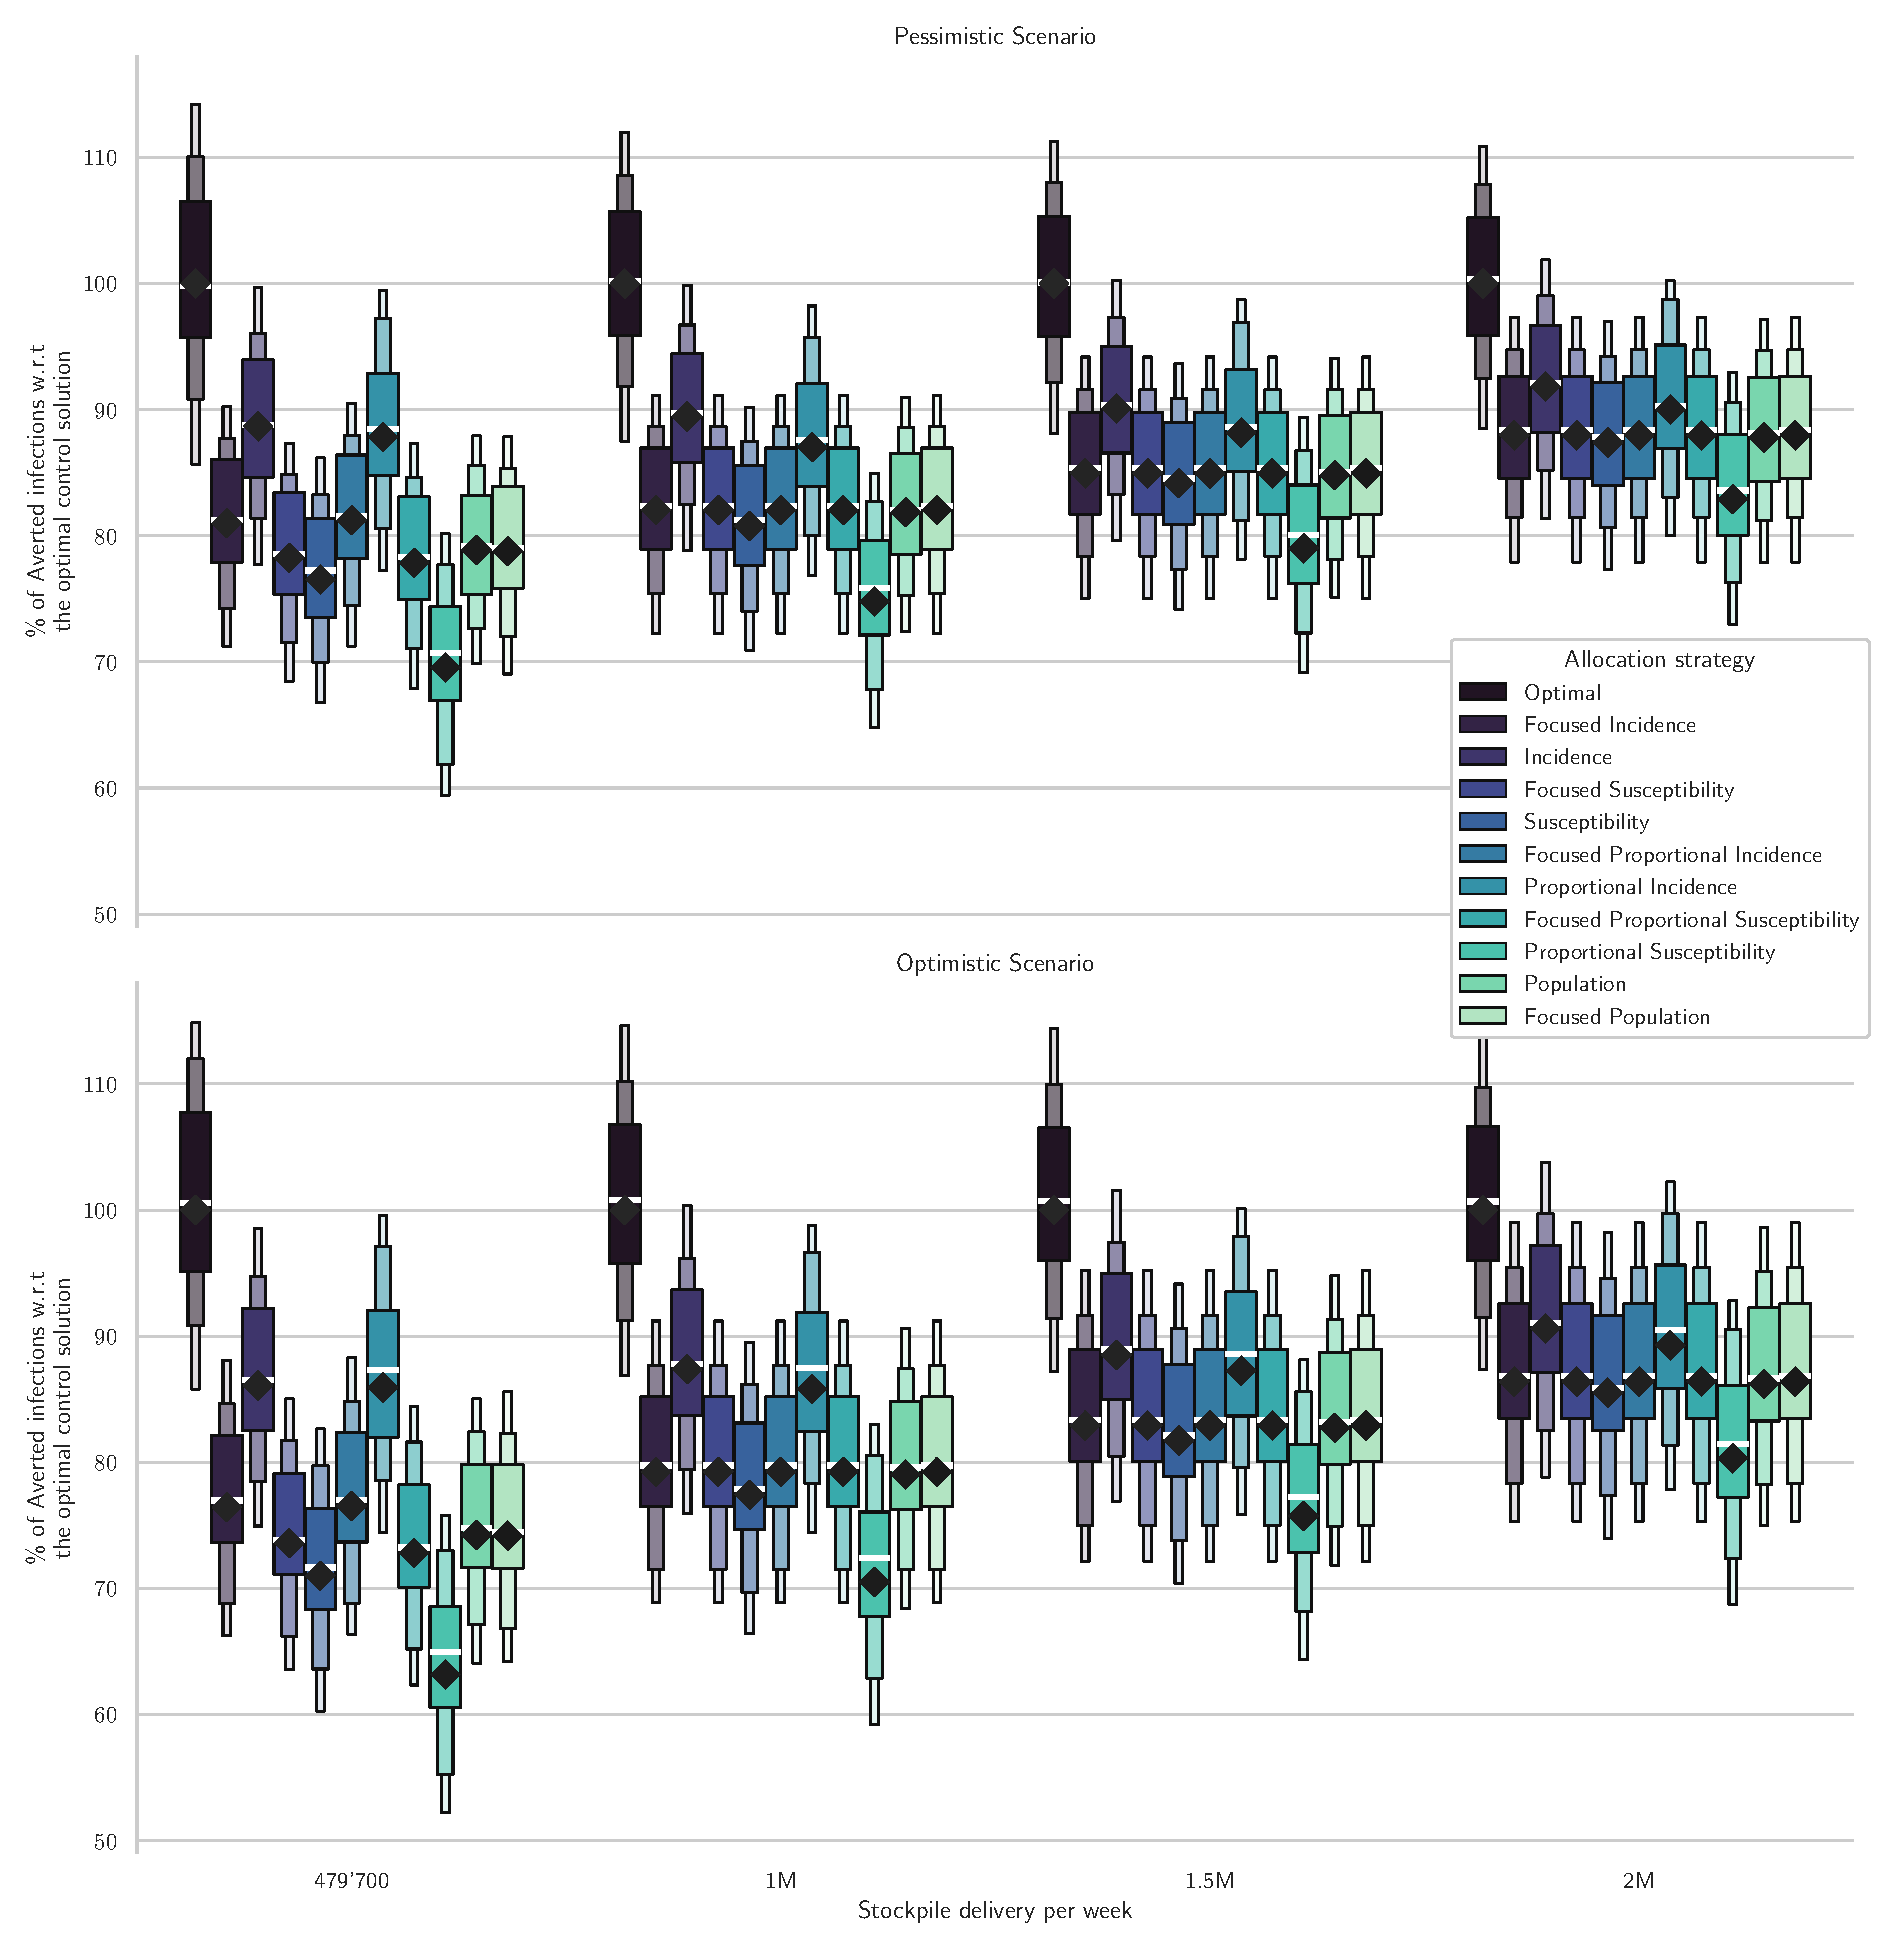
\includegraphics[width=0.9\textwidth]{fig_italy-ocp/figuresSI/scenarios_perturb_all_SI.pdf}
    \caption[Comparison of different allocation strategies]{Comparison of different allocation strategies. Percentages of averted infections per vaccine dose from January 11, 2021 to April 11, 2021 using different vaccine distribution strategies for the pessimistic (panel A) and the optimistic (panel B) scenario based on: the optimal solution, the spatial distribution of the population, the amount of susceptible individuals at the beginning of the vaccination campaign, and the projected disease incidence in the absence of control. We optimize a median realization of the modeled posterior (diamonds), and assess the performance on the whole posterior (box plots). The results are normalized by the number of averted infections in the optimized solution (see Table \ref{table:all_strat} for absolute values).}
    \label{fig:OC_comparison_all}
\end{fwfigure}


\begin{figure}[!ht]
    \centering
    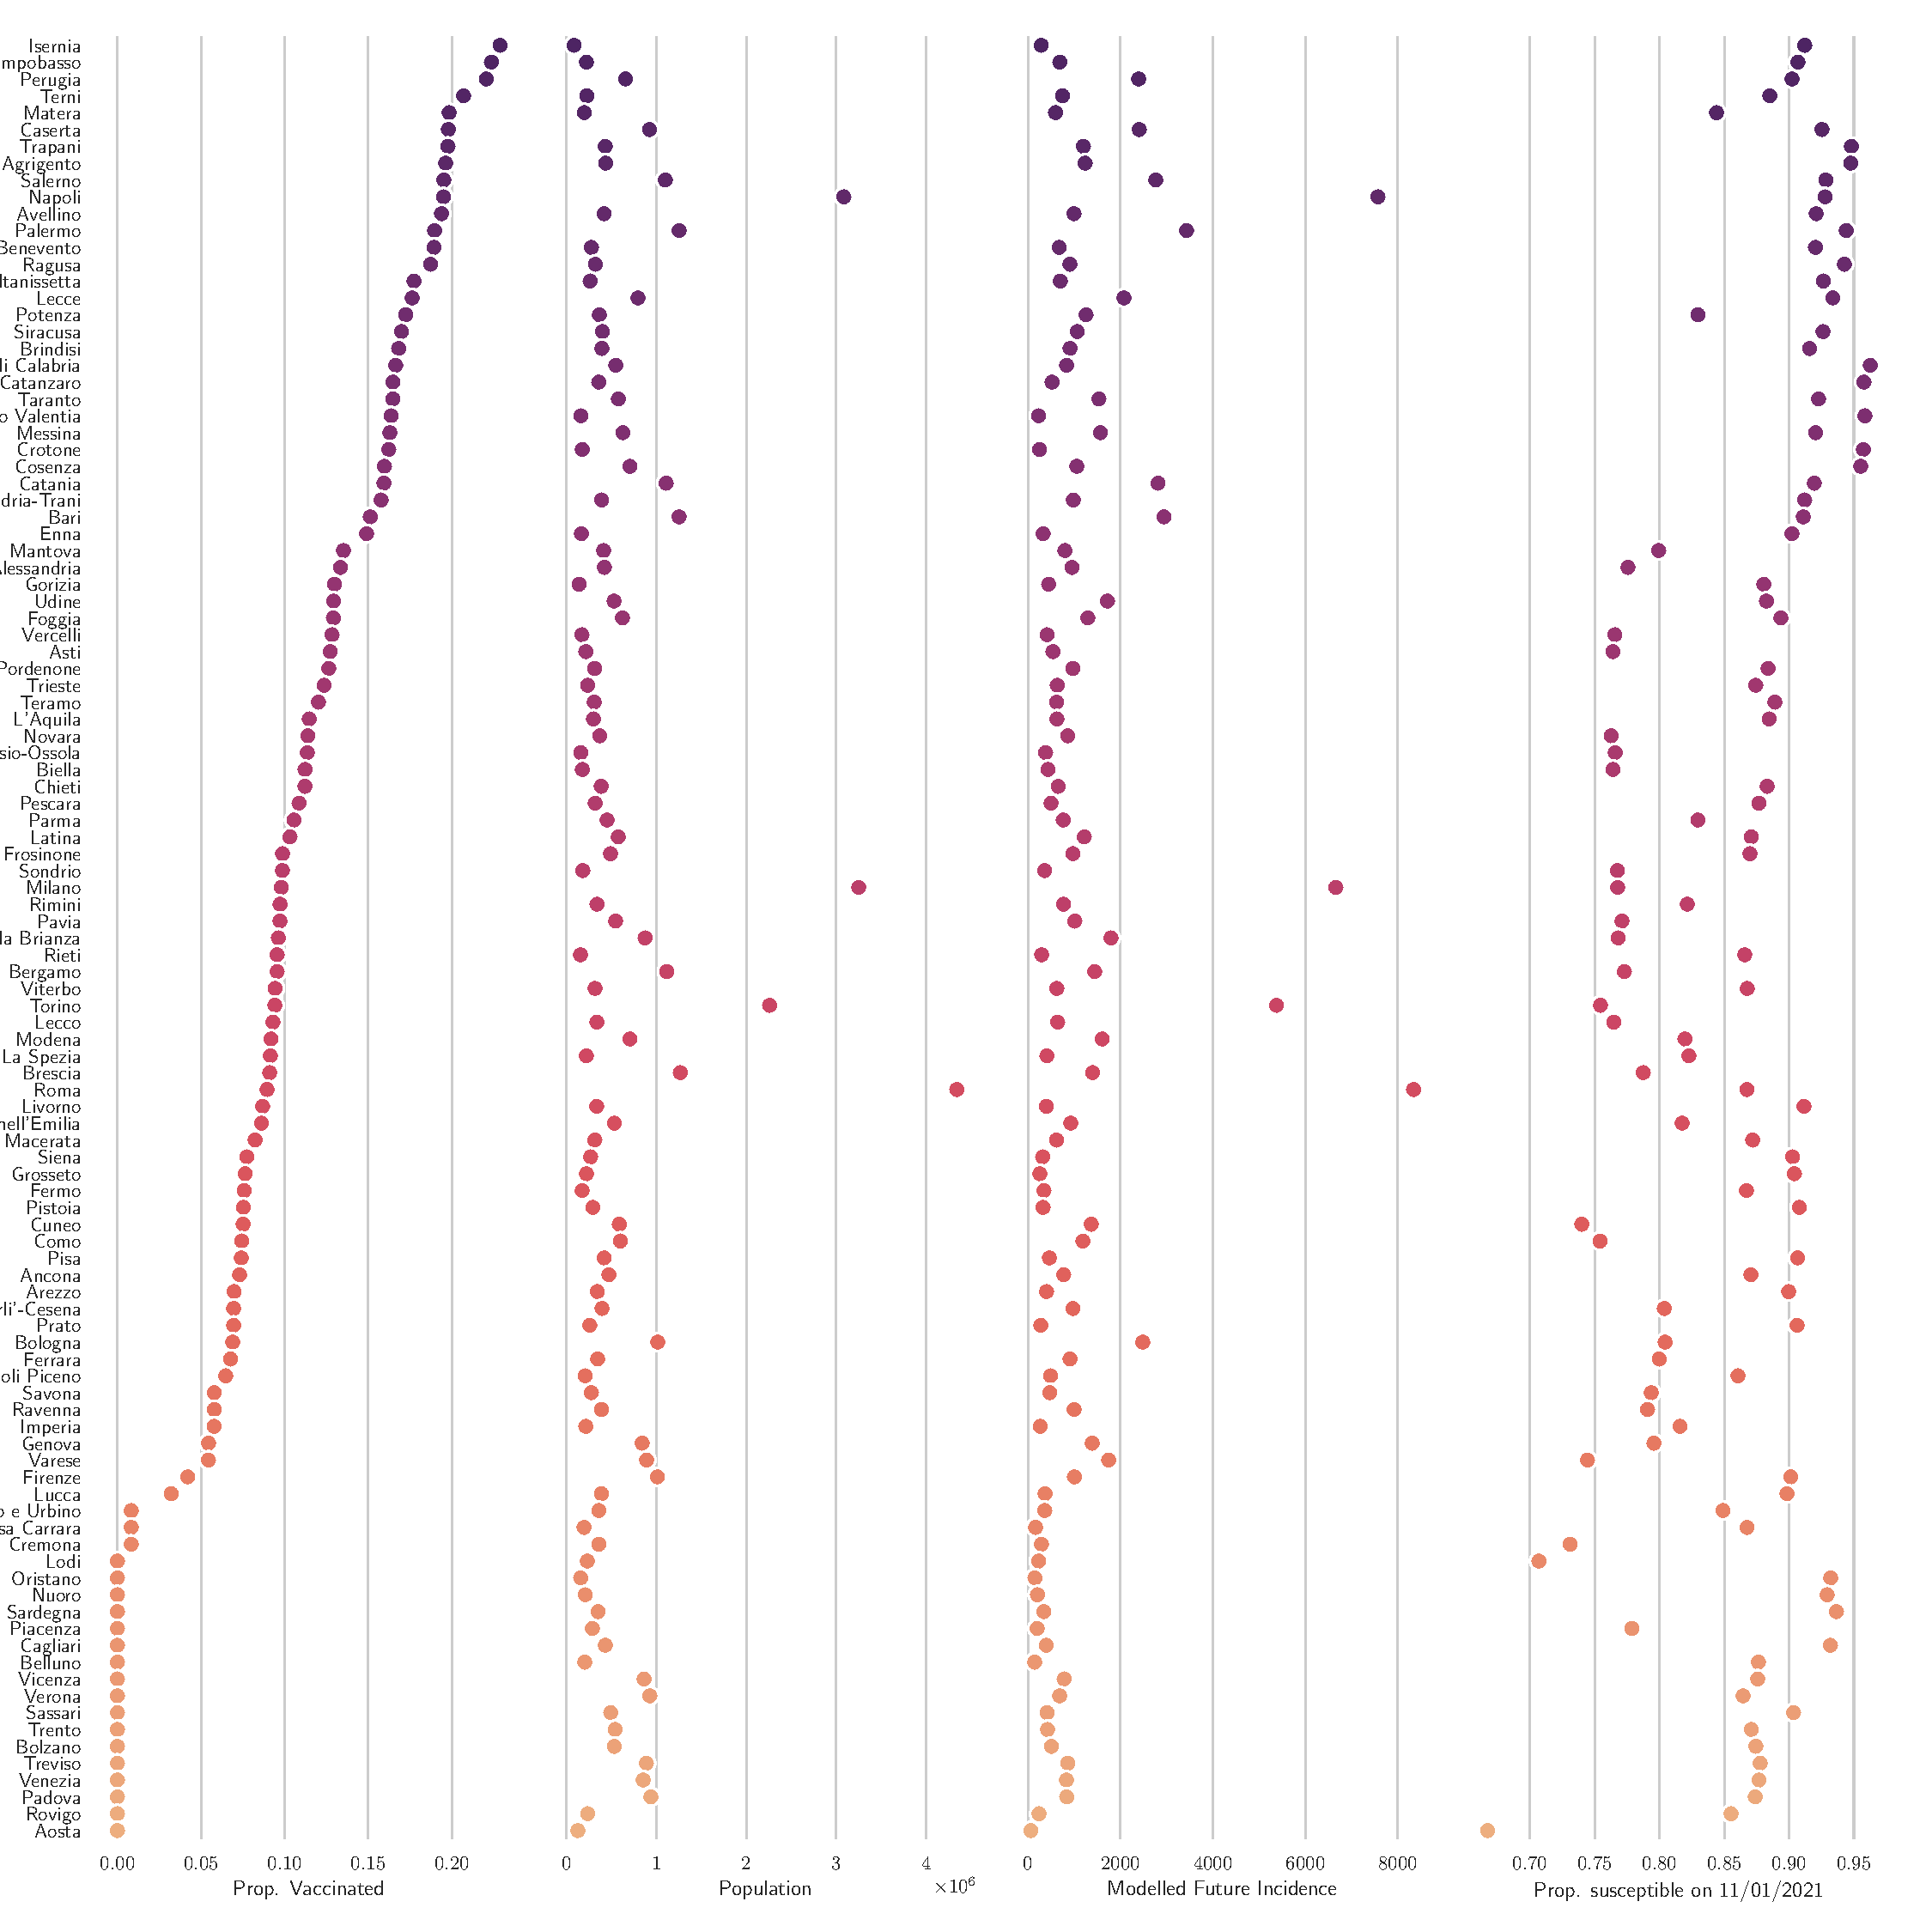
\includegraphics[width=\textwidth]{fig_italy-ocp/figuresSI/SI_scatter_Optimistic.pdf}
    \caption[Control and co-variates for the optimistic scenario]{Control and co-variates for the optimistic scenario with a stockpile delivery of 479'700 vaccine doses.}
    \label{fig:OC_scatter_optimistic}
\end{figure}

\begin{figure}[!ht]
    \centering
    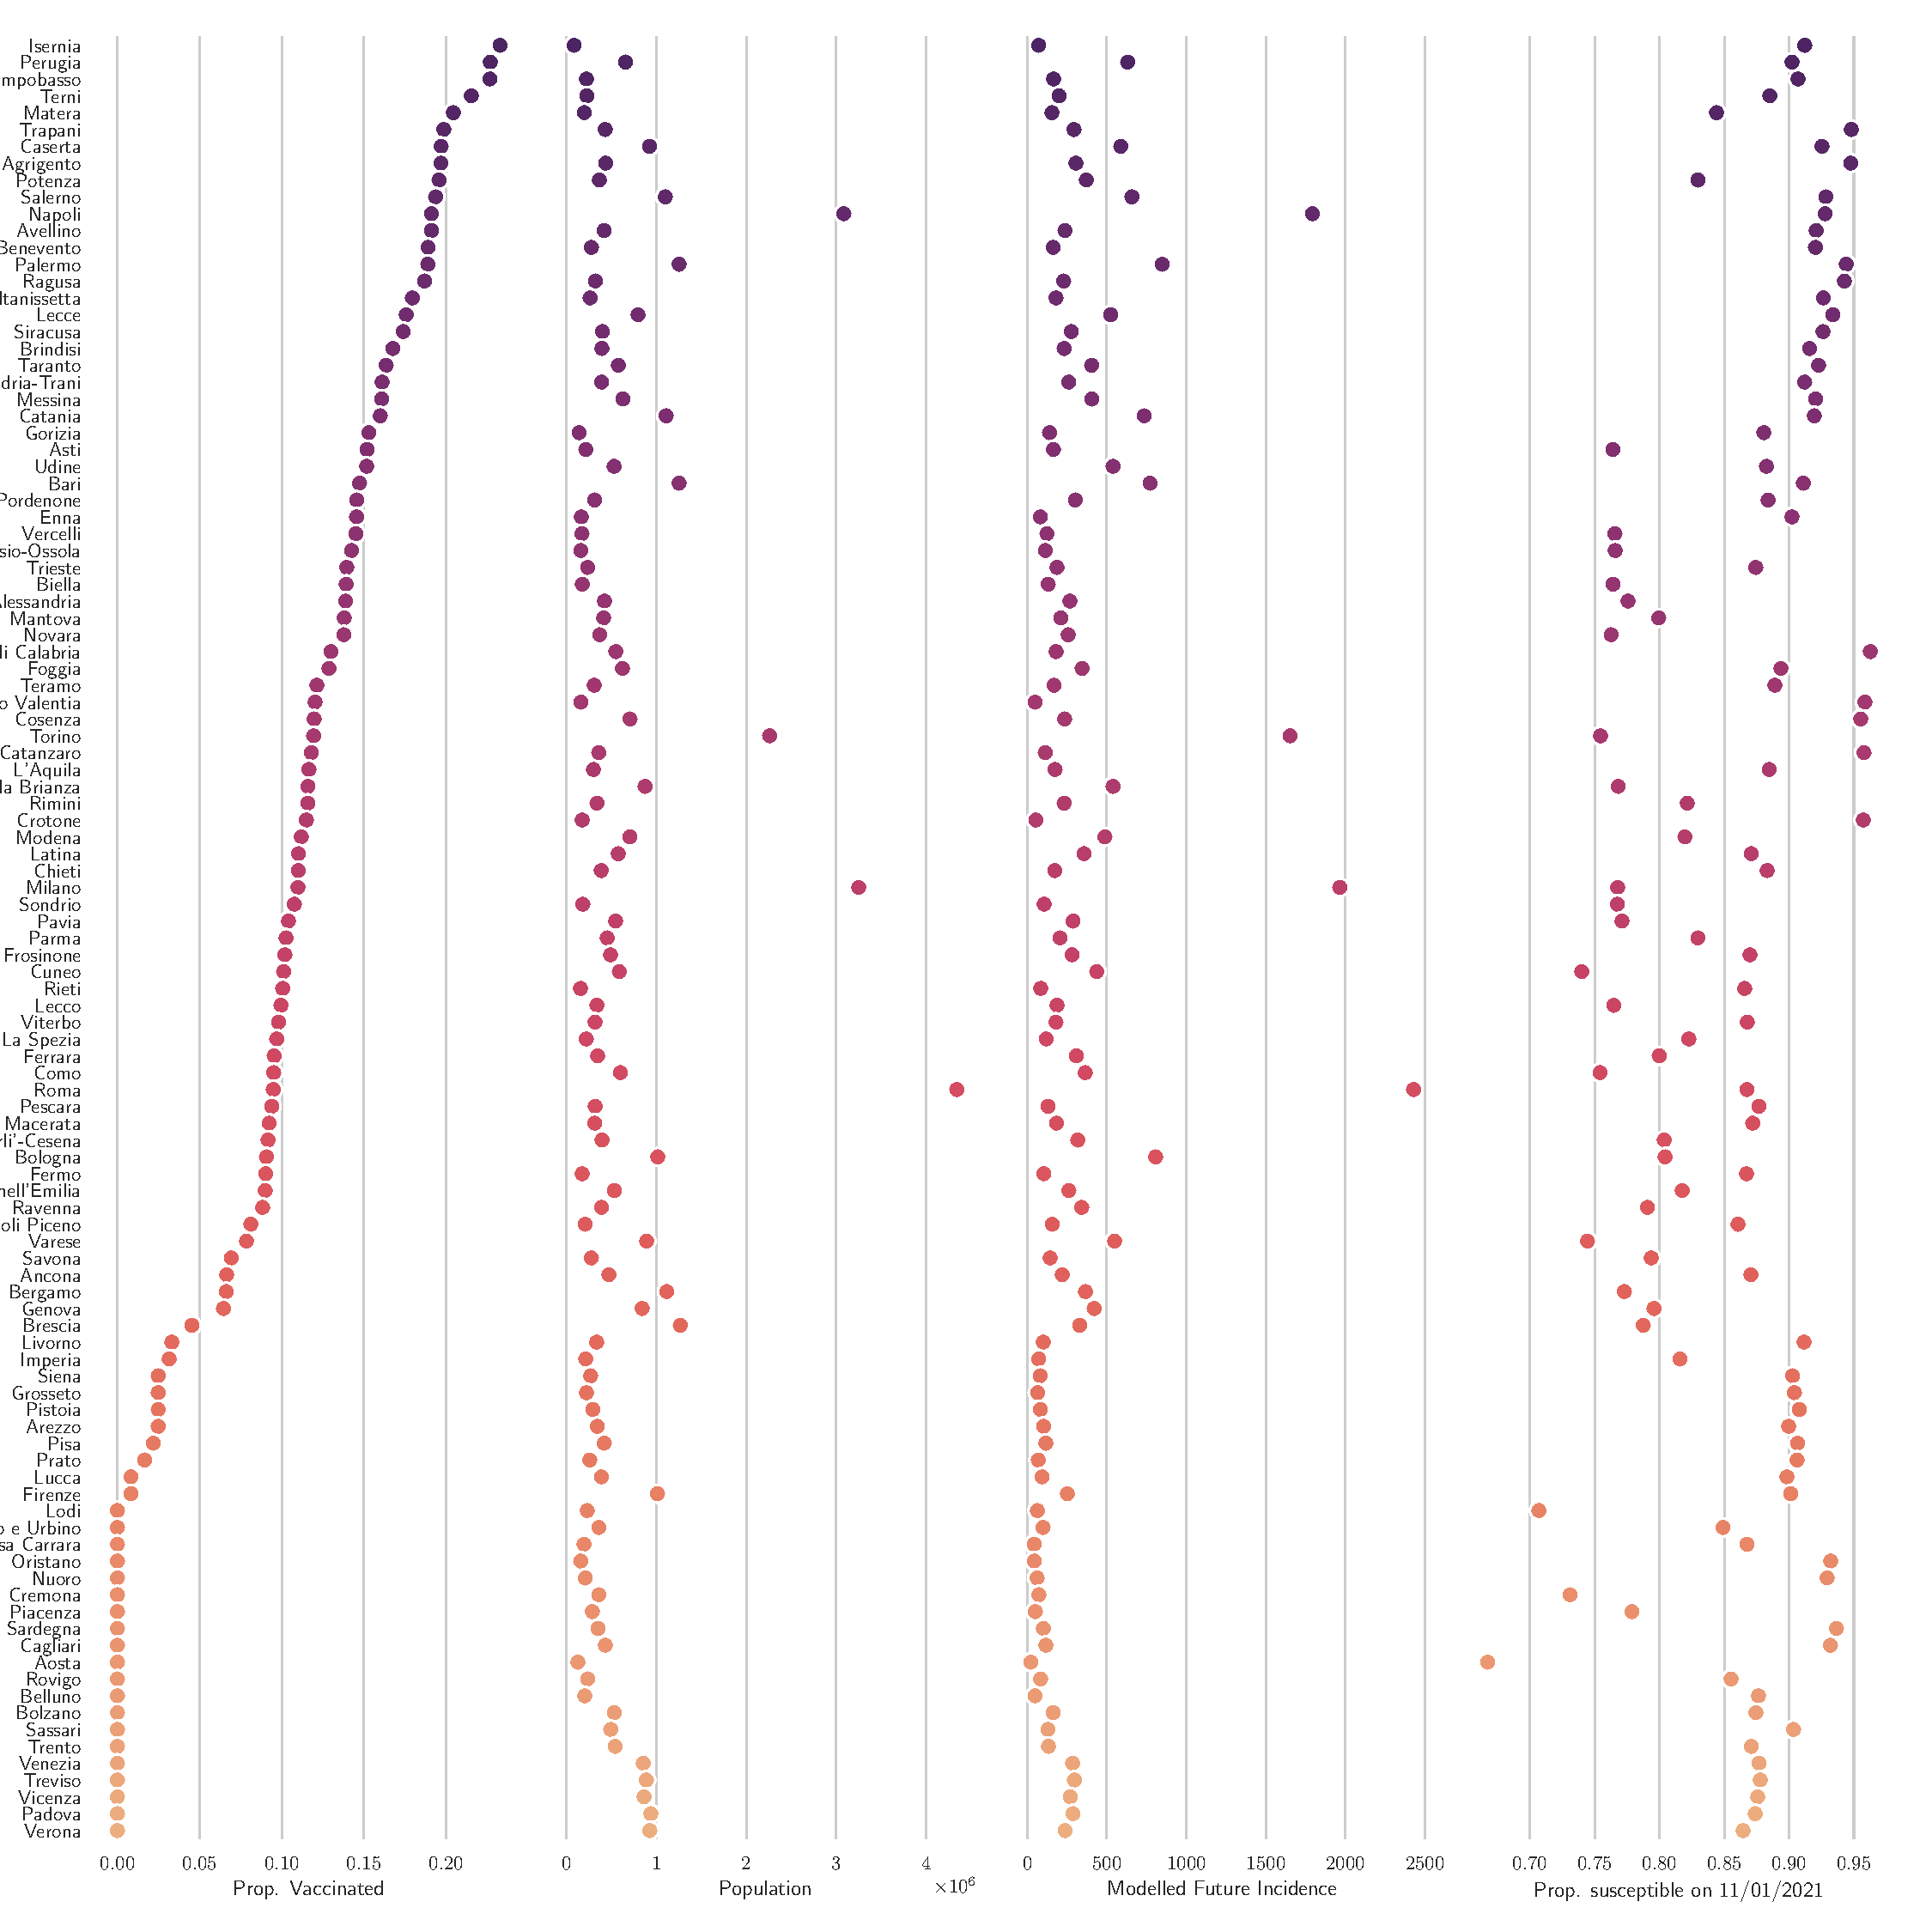
\includegraphics[width=\textwidth]{fig_italy-ocp/figuresSI/SI_scatter_Pessimistic.pdf}
    \caption[Control and co-variates for the pessimistic scenario]{Control and co-variates for the pessimistic scenario with a stockpile delivery of 479'700 vaccine doses.}
    \label{fig:OC_scatter_pessimistic}
\end{figure}

%\begin{figure}[!ht]
%    \centering
 %   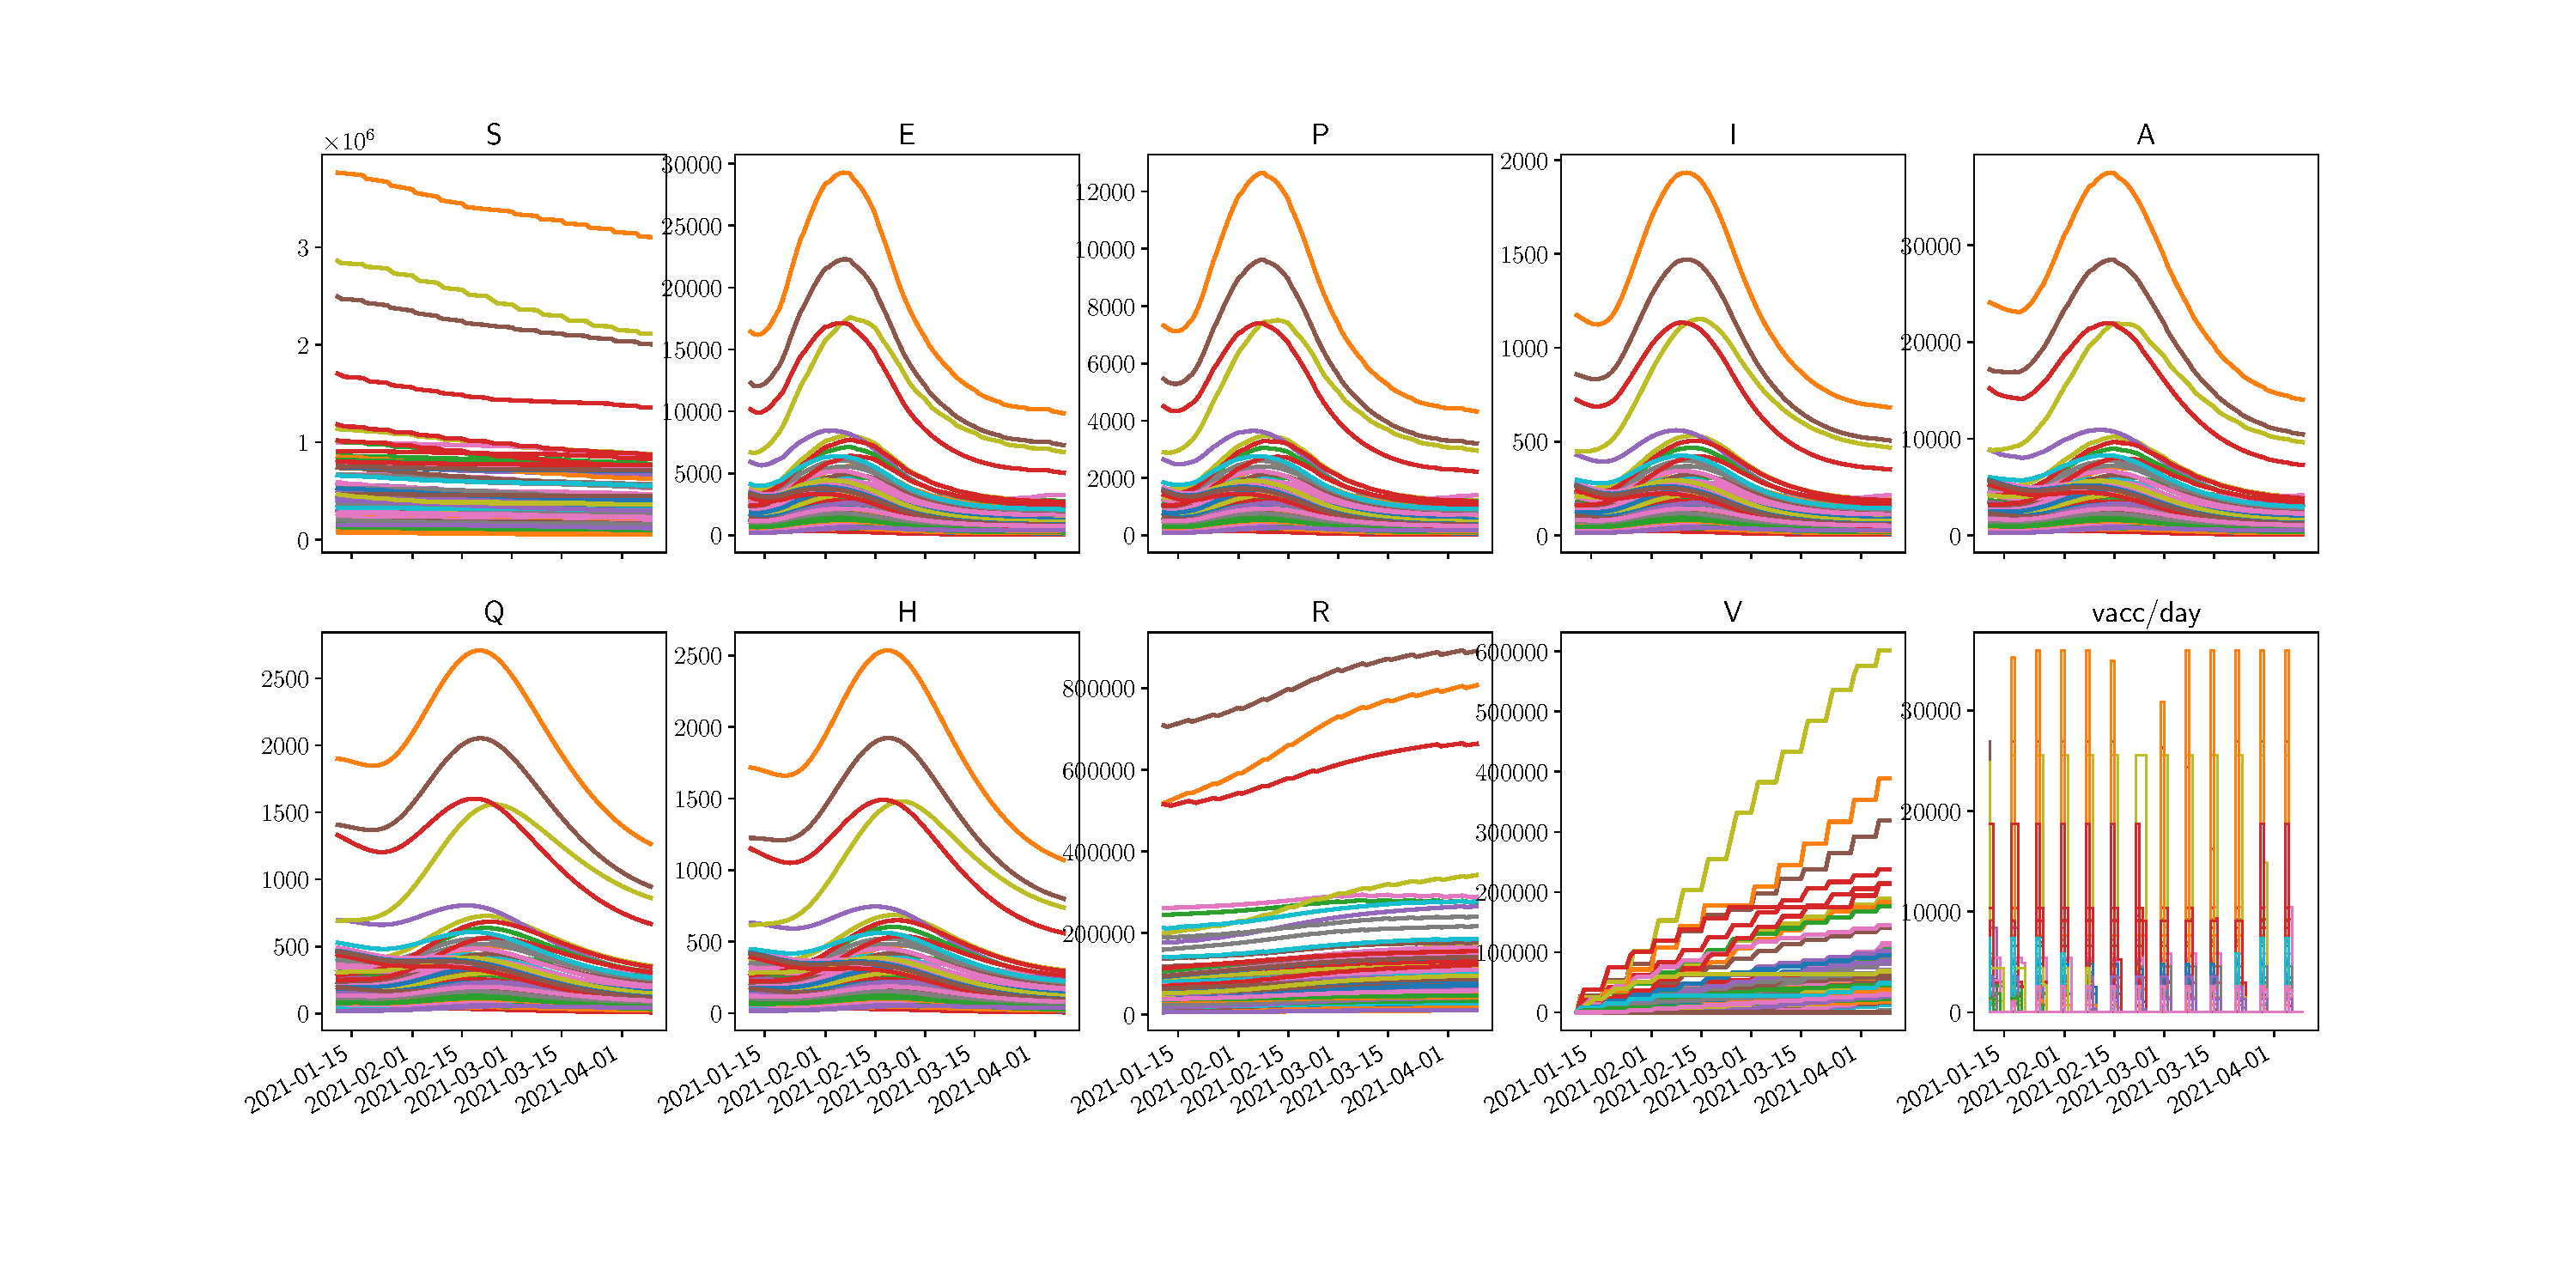
\includegraphics[width=\textwidth]{fig_italy-ocp/figuresSI/SI_all_states.pdf}
  %  \caption[Example of the dynamics in all compartments]{Example of the dynamics in all compartments for every node in the pessimistic scenario with a stockpile delivery of 479'700 doses. The lower right plot shows the control variable, the number of doses per day in each province.}
%    \label{fig:OC_ts_all}
%\end{figure}




